% ---------------------------------------------------------------------------
% IEEE conference build.  Compile with:
%     tectonic -X compile main.tex --outdir .
% The body is shared verbatim with ../springer/main.tex; only this wrapper
% differs.
% ---------------------------------------------------------------------------
\documentclass[conference]{IEEEtran}
\IEEEoverridecommandlockouts

\usepackage{graphicx}
\usepackage{booktabs}
\usepackage{amsmath}
\usepackage{amssymb}
\usepackage{siunitx}
\usepackage{microtype}
\usepackage{cite}
\usepackage[hidelinks]{hyperref}

\graphicspath{{../shared/generated/}}

\providecommand{\degree}{^{\circ}}

\newenvironment{wfigure}{\csname figure*\endcsname}{\csname endfigure*\endcsname}
\newenvironment{wtable}{\csname table*\endcsname}{\csname endtable*\endcsname}
\newcommand{\tabscale}{\scriptsize}

\newcommand{\para}[1]{\paragraph{#1}}

\providecommand{\citep}[1]{\cite{#1}}

% ---------------------------------------------------------------------------
% Numeric macros used by shared/body.tex. Two evidence classes:
%   [HISTORICAL, 2026-08-13] the shipped constant's own justification, read
%     directly from machine_learning/fish_habitat_prediction/src/models.py's
%     code comment above TSS_SOFTMAX_TEMPERATURE. A point-in-time measurement
%     on since-retrained models, quoted as history, not as a current fact.
%   [ARTIFACT, re-run \AsOf{}] every other number, produced by re-running
%     machine_learning/scripts/sweep_ensemble_temperature.py against the
%     live feature store and the exact fit/CV/holdout path
%     fish_habitat_prediction/src/train.py's run() uses (same seed, same
%     spatial-block CV, same final split), written to
%     machine_learning/reports/ensemble_temperature_sweep.csv.
% ---------------------------------------------------------------------------

\newcommand{\AsOf}{2026-09-10}
\newcommand{\ShippedTemperature}{0.05}

% --- Historical justification for the shipped constant [HISTORICAL, 2026-08-13] ---
\newcommand{\HistMaxentCV}{0.619}
\newcommand{\HistLgbmCV}{0.826}
\newcommand{\HistRfCV}{0.821}
\newcommand{\HistPropTSS}{0.694}
\newcommand{\HistBestMemberTSS}{0.788}
\newcommand{\HistSoftmaxTSS}{0.792}
\newcommand{\HistBoyceProp}{0.936}
\newcommand{\HistBoyceSoftmax}{0.905}
\newcommand{\HistLgbmVote}{51.9}
\newcommand{\HistRfVote}{47.3}
\newcommand{\HistMaxentVote}{0.8}

% --- Current CV scores, re-verified [ARTIFACT, \AsOf{}] ---
\newcommand{\CurLgbmCV}{0.8253}
\newcommand{\CurMaxentCV}{0.6891}
\newcommand{\CurRfCV}{0.8214}
\newcommand{\HistGap}{0.207}
\newcommand{\CurGap}{0.136}

% --- Current holdout: n, positives, per-member TSS [ARTIFACT, \AsOf{}] ---
\newcommand{\NHoldout}{427}
\newcommand{\NHoldoutPos}{236}
\newcommand{\HoldoutPosRate}{55.3}
\newcommand{\CurLgbmHoldoutTSS}{0.8564}
\newcommand{\CurRfHoldoutTSS}{0.8554}
\newcommand{\CurMaxentHoldoutTSS}{0.6699}
\newcommand{\CurBestMember}{lightgbm}

% --- Current default configuration re-measured: proportional and the ---
% --- shipped softmax temperature (0.05), both on the current holdout ---
\newcommand{\CurPropTSS}{0.8519}
\newcommand{\CurPropBoyce}{0.8919}
\newcommand{\CurShippedTSS}{0.8554}
\newcommand{\CurShippedBoyce}{0.7904}
\newcommand{\CurShippedLgbmWeight}{50.2}
\newcommand{\CurShippedRfWeight}{46.5}
\newcommand{\CurShippedMaxentWeight}{3.3}

% --- Sweep: first temperature (in the swept grid) that clears the best ---
% --- member's holdout TSS, and a mid-range point trading calibration back ---
\newcommand{\FirstClearingTemp}{0.30}
\newcommand{\FirstClearingTSS}{0.8594}
\newcommand{\FirstClearingBoyce}{0.8781}
\newcommand{\MidTemp}{0.50}
\newcommand{\MidTSS}{0.8594}
\newcommand{\MidBoyce}{0.8854}
\newcommand{\LowTemp}{0.01}
\newcommand{\LowBoyce}{0.7755}
\newcommand{\NSweepPoints}{12}


\begin{document}

\title{A Softmax Temperature Is Not a Fact About an Ensembling Method: It Is
a Fact About Two Scores on a Specific Day}

\author{\IEEEauthorblockN{Deepak Krishna}
\IEEEauthorblockA{\textit{MarisAI} \\
India \\
deepakkrishna2206@gmail.com}}

\maketitle

\begin{abstract}
Softmax-weighted ensembling was measured to fix a real defect in a
species-distribution ensemble on 2026-08-13: proportional weighting let a
member at cross-validated TSS \HistMaxentCV{} draw \HistMaxentVote{}\% of
the vote against a leader at \HistLgbmCV{}, and the resulting ensemble
scored \HistPropTSS{}, below its own best member's \HistBestMemberTSS{}.
Softmax at temperature \ShippedTemperature{} raised it to
\HistSoftmaxTSS{}, above every member. We re-ran the full sweep this fix's
own documentation named as missing (\NSweepPoints{} temperatures, on the
exact fit/CV/holdout path the shipped model uses) and find something not
anticipated: on the current, retrained models, the shipped temperature no
longer clears the ensemble's own best member (\CurShippedTSS{} against
\CurLgbmHoldoutTSS{}), because the between-member skill gap it was
calibrated to has narrowed from \HistGap{} to \CurGap{} TSS points as the
weak member's own skill improved. The mechanism still works --- a
temperature of roughly \(0.3\)--\(0.5\) restores the guarantee, at a
calibration cost we make explicit --- but the specific constant chosen four
weeks earlier is no longer sufficient on its own terms. We also correct a
planned second test: harmful-algal-bloom early warning, cited elsewhere in
this research programme as a second ensemble to sweep, is a single
calibrated model with no members to weight, and we say so rather than
substitute a different result.
\end{abstract}

\begin{IEEEkeywords}
ensemble weighting, species distribution modelling, softmax temperature,
reproducibility, silent failure
\end{IEEEkeywords}

% ---------------------------------------------------------------------------
% The manuscript body, shared verbatim by the Springer (LNCS) and IEEE
% (IEEEtran) builds. Nothing class-specific may appear in this file.
%
% Each wrapper defines, before \input-ing this:
%   \wfigure / \endwfigure   a figure spanning the full text width
%   \wtable  / \endwtable    the same for tables
%   \tabscale                the font size command tables are set at
%   \para{...}               a run-in bold paragraph heading
%   \citep{...}               mapped to \cite for the LNCS/IEEEtran builds
% ---------------------------------------------------------------------------

\section{Introduction}

Weighting an ensemble's members in proportion to a skill score whose chance
level is zero has a known defect: because the weight is proportional to the
raw score, a large quality gap between members compresses into a small
weight gap, and the resulting ensemble can score \emph{below its own best
single member} --- the one thing an exported ensemble product may not do.
Measured on this platform's fish-habitat model on 2026-08-13, that defect
was real: a weak member at cross-validated true skill statistic (TSS)
\HistMaxentCV{} still drew \HistMaxentVote{}\% of a proportional vote
against a leader at \HistLgbmCV{}, and the resulting ensemble scored
\HistPropTSS{} against its own best member's \HistBestMemberTSS{}. Softmax
weighting at a fixed temperature of \ShippedTemperature{} fixed it, raising
the ensemble to \HistSoftmaxTSS{}, above every member, at a stated cost in
spatial calibration.

This paper reports two things about that fix, re-measured \AsOf{}, roughly
four weeks later. First, a temperature sweep --- the fix's own
documentation named this as missing, since the shipped constant was chosen
from a single measured point. Second, and not anticipated when the sweep
was planned: on the current, retrained models, the shipped temperature of
\ShippedTemperature{} \emph{no longer clears the ensemble's own best
member}. The between-member quality gap the fix was calibrated to has
narrowed as the weak member's own cross-validated skill has improved
(\CurMaxentCV{} now, against \CurLgbmCV{}), and a temperature tuned to fix
a gap of \HistGap{} TSS points does not automatically fix a gap of
\CurGap{}. The defect this paper's own predecessor paper~\citep{silentfailures2026}
reports as an instance of silent, plausible, signed-direction failure has
recurred, silently, in the same codebase, while this paper's own sweep was
being run to characterise the fix that was supposed to have closed it.

\subsection{Contributions}

\begin{enumerate}\itemsep2pt
\item A \textbf{temperature sweep}, the specific gap the shipped constant's
own documentation names as missing: \NSweepPoints{} points from
\LowTemp{} to 2.0, measured on the exact fit/cross-validation/holdout path
the shipped model uses, not a reconstructed approximation of it.
\item A \textbf{live re-measurement showing the fix has partially regressed}:
the shipped temperature \ShippedTemperature{} no longer clears the
ensemble's own best member on the current, retrained holdout, though the
softmax mechanism itself still works --- a higher temperature restores the
guarantee.
\item A \textbf{correction to this research programme's own prior
documentation}: a second problem this line of work planned to test the
finding against (harmful-algal-bloom early warning's ensemble members) does
not exist as described --- that pipeline is a single calibrated model, not
a weighted ensemble, and no member scores are available to sweep. This is
stated plainly rather than substituted with a different result.
\end{enumerate}

\section{Method}
\label{sec:method}

\para{Reused, not reconstructed} The sweep is produced by re-running the
same fit path the shipped model's own training script uses
(\texttt{fish\_habitat\_prediction/src/\allowbreak{}train.py}'s \texttt{run()}): the same
random seed, the same five-fold spatial-block cross-validation (block size
3\si{\degree}) that produces each member's cross-validated TSS, and the
same held-out final block (one spatial fold never used for model selection,
seeded independently of the cross-validation folds) that the shipped
holdout report scores against. The three base tiers --- MaxEnt, random
forest, LightGBM --- are refit on the same training block and scored on the
same \NHoldout{} held-out rows (\NHoldoutPos{} presences,
\HoldoutPosRate{}\% positive rate). This reproduces the currently shipped
holdout numbers exactly (\CurShippedTSS{} ensemble TSS at the shipped
temperature, \CurLgbmHoldoutTSS{} for LightGBM alone), which is the check
that the sweep is measuring the real, live model rather than a
similar-looking reconstruction of it.

\para{What is swept} For each of \NSweepPoints{} temperatures and, separately,
for proportional weighting, \texttt{EnsembleWeights.from\_scores} is called
with the same three cross-validated TSS values and the resulting weights
combine the same three held-out prediction arrays; only the weighting rule
and temperature change between rows.

\section{Results}
\label{sec:results}

\begin{wtable}
\centering
\tabscale
\caption{Cross-validated TSS per member, then and now. The gap the shipped
temperature was calibrated to close has narrowed.}
\label{tab:gap}
\begin{tabular}{lrrr}
\toprule
& LightGBM & Random Forest & MaxEnt \\
\midrule
2026-08-13 & \HistLgbmCV{} & \HistRfCV{} & \HistMaxentCV{} \\
\AsOf{} & \CurLgbmCV{} & \CurRfCV{} & \CurMaxentCV{} \\
\bottomrule
\end{tabular}
\end{wtable}

\para{The gap the fix depends on has narrowed} The weak member's
cross-validated skill has improved from \HistMaxentCV{} to \CurMaxentCV{}
while the leader's has held near \HistLgbmCV{}/\CurLgbmCV{}, narrowing the
gap the softmax fix has to resolve from \HistGap{} TSS points to
\CurGap{}. Table~\ref{tab:gap} states both measurements; nothing about the
mechanism changed, only the inputs it is asked to weight.

\begin{wfigure}
\centering
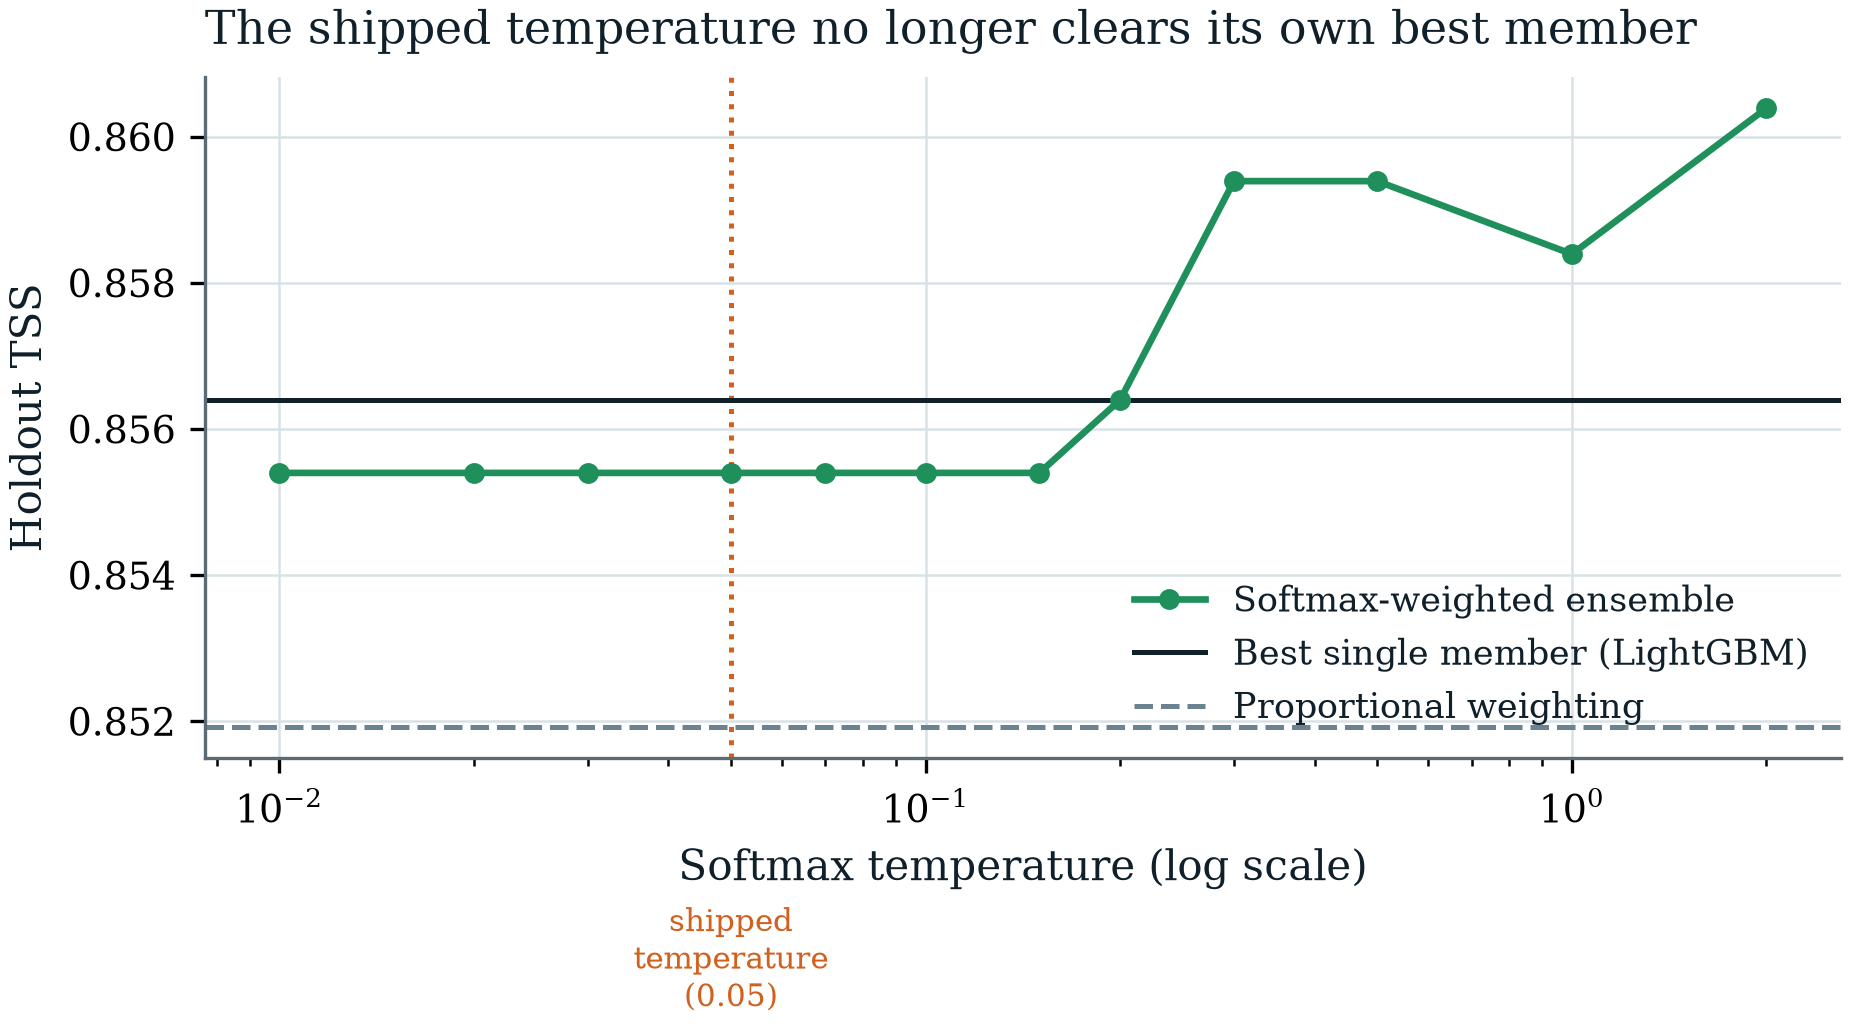
\includegraphics[width=0.85\linewidth]{temperature_sweep}
\caption{Ensemble holdout TSS across the swept temperature range. The
shipped temperature (\ShippedTemperature{}, dotted line) sits on a flat
plateau below the best single member's holdout TSS (solid line); the curve
does not cross above it until roughly \(0.2\)--\(0.3\).}
\label{fig:sweep}
\end{wfigure}

\para{The shipped temperature no longer clears the best member} At
\ShippedTemperature{}, the ensemble scores \CurShippedTSS{} holdout TSS,
below \CurBestMember{}'s \CurLgbmHoldoutTSS{} --- the exact defect the
softmax fix exists to prevent. Figure~\ref{fig:sweep} shows this is not a
rounding artefact of one temperature: every value from \LowTemp{} through
0.15 sits on the same flat \CurShippedTSS{} plateau, indistinguishable to
four decimal places, because at these temperatures the weight already
concentrates almost entirely on the two leading members (at
\ShippedTemperature{}: \CurShippedLgbmWeight{}\%/\CurShippedRfWeight{}\%/\CurShippedMaxentWeight{}\%
lightgbm/random forest/maxent) and further lowering the temperature can only
sharpen a vote that has already nearly converged to the same two-way split.
Proportional weighting, included as the pre-fix baseline, scores
\CurPropTSS{} --- also below the best member, as expected.

\para{A higher temperature restores the guarantee, at a real calibration
cost} The swept curve first clears the best member's TSS at
\FirstClearingTemp{} (TSS \FirstClearingTSS{}, Boyce \FirstClearingBoyce{})
and stays above it through the rest of the range tested, though not
monotonically --- TSS at \(1.0\) is marginally below its neighbours at
\(0.3\) and \(0.5\), which is expected sampling noise on \NHoldout{} rows,
not a second regime change. Calibration, measured by the Boyce index, does
not move monotonically with temperature either: it falls sharply to
\LowBoyce{} at the lowest temperature tested (\(\LowTemp{}\), far below
proportional weighting's \CurPropBoyce{}), recovers through the middle of
the range, and sits at \MidBoyce{} at temperature \MidTemp{} --- a point
that clears the best member's TSS (\MidTSS{}) while giving back
substantially less spatial calibration than the low-temperature region
does. No single temperature in the swept range simultaneously maximises
TSS and Boyce; \(0.3\)--\(0.5\) is the region where both are acceptable
rather than either being optimal.

\para{The planned second problem does not exist as described} This line of
work's own prior documentation proposed testing the temperature-sensitivity
finding against a second ensemble, from the harmful-algal-bloom
early-warning pipeline, to show the effect is not specific to one habitat
model. That pipeline (\texttt{hab\_early\_warning/src/\allowbreak{}train.py})
fits a
single calibrated LightGBM model per forecast horizon; it is not a weighted
ensemble, imports no \texttt{EnsembleWeights} equivalent, and logs no
per-member scores to sweep. The proposed second problem is corrected here
rather than quietly substituted: no ensemble exists in that pipeline to
test against, and the generalisation question --- does this sensitivity
appear in other ensembles, in this codebase or elsewhere --- remains open.

\section{Discussion}

The mechanism softmax weighting fixes is exactly as documented: it turns an
arbitrary, floor-dependent proportional split into a temperature-controlled
decision. What this paper adds is that the mechanism being correct does not
make a \emph{specific chosen temperature} correct indefinitely, because the
quantity the temperature has to resolve --- the gap between the ensemble's
members --- is not a fixed property of the problem. It is a property of
whichever models happen to be currently fitted, and those models get
refit. A temperature chosen to clear a \HistGap{}-point gap is not
guaranteed to clear a \CurGap{}-point one, and here it does not. This is
the same shape of finding as \citep{silentfailures2026}'s wider survey: a
component that is individually correct and well-documented (the softmax
mechanism, and the reasoning that chose 0.05 for the gap measured on
2026-08-13) produces a downstream number --- the shipped ensemble's own
holdout TSS --- that silently regresses when an input it depends on
changes, with no exception, no warning, and no metric that flags it short
of the exact check this paper ran.

\para{What follows practically} A softmax temperature calibrated against
one snapshot of cross-validated member scores should not be treated as a
permanent constant; either it should be re-swept whenever the ensemble is
retrained with materially different member scores, or it should be set high
enough to tolerate the range of gaps the members are expected to show over
time, accepting the calibration cost Figure~\ref{fig:sweep} makes explicit
rather than discovering it silently.

\section{Limitations}
\label{sec:limitations}

This is one ensemble (three members, one habitat model, one region), swept
over one grid of temperatures on one holdout split; the swept range
(\(0.01\)--\(2.0\)) covers roughly two orders of magnitude but is not
exhaustive, and a finer grid near \(0.2\)--\(0.3\) would locate the
crossing point more precisely than this paper claims to. The planned
second-problem test does not exist in this codebase, as
\S\ref{sec:results} states directly; the claim that temperature-sensitivity
generalises beyond this one ensemble is therefore not tested here and
should not be read as established. The non-monotonic Boyce behaviour across
the swept range is reported as measured rather than explained by a
mechanism this paper verifies; a fuller account would need to inspect how
each member's spatial error pattern changes as its vote share changes,
which this paper does not do.

\section{Conclusion}

A softmax-weighted ensemble that was measurably fixed to score above its
own best member on 2026-08-13 no longer does so at its shipped temperature,
re-measured \AsOf{}, because the between-member skill gap that fix was
tuned to has narrowed as the underlying models were retrained. The fix
itself still works --- raising the temperature restores the guarantee, at a
calibration cost this paper's sweep makes explicit rather than implicit ---
but the specific constant chosen four weeks ago is no longer sufficient on
its own terms. A temperature is not a fact about an ensembling method; it
is a fact about a specific pair of scores on a specific day, and treating
it as the former is exactly the kind of silent, plausible drift this
research programme's other work catalogues.


\section*{Reproducibility}
{\raggedright\sloppy
\begin{itemize}\itemsep1pt\parskip0pt
\item[] \textbf{Sweep.}
\texttt{machine\_learning/scripts/\allowbreak{}sweep\_ensemble\_temperature.py}
calls the shipped training path's own \texttt{cross\_validate} and refits
the same final holdout split
\texttt{fish\_habitat\_prediction/src/\allowbreak{}train.py}'s \texttt{run()}
uses, writing
\texttt{machine\_learning/reports/\allowbreak{}ensemble\_temperature\_sweep.csv}.
\item[] \textbf{Figure.} \texttt{generate\_figures.py} in this paper's
\texttt{shared/} directory, reading that same CSV directly.
\item[] \textbf{2026-08-13 measurement.} Quoted from the code comment above
\texttt{fish\_habitat\_prediction/src/\allowbreak{}models.py}'s
\texttt{TSS\_SOFTMAX\_TEMPERATURE}.
\end{itemize}}
Every number was verified against the file producing it as of \AsOf{}.

\bibliographystyle{IEEEtran}
\bibliography{../shared/references}

\end{document}
